% kapitel2.tex
\chapter{Der Aufbau und die Fertigung}
\label{chapter:kap1}
\section{Die technischen Komponenten}
In Tabelle 2.1 listen wir die von uns verbauten Komponenten auf. \\
Wir werden diese in den darauf folgenden Unterkapiteln näher beschreiben und uns dazu äußern weshalb wir uns für genau diese Bauteile entschieden haben. Die Komponenten teilen sich im großen und ganzen in zwei Komponentengruppen auf. Die Gruppe die für die Herstellung des Spiegels selbst notwendig ist und die Gruppe, welche im Spiegel verbaut wird und somit dem Spiegel seine Funktionalität ermöglicht.
\begin{table}[H]
	\small
	\begin{tabular}{r|l|l|r}
		& \textbf{Komponente} & \textbf{Link} & \textbf{Preis €} \\
		\hline
		\multirow{4}{*}{\textbf{Spiegeleinheit}} & IKEA RIBBA Rahmen, schwarz &
		\href{http://www.ikea.com/de/de/catalog/products/00078051/#/20078050}{IKEA} & 12,99 \\
		& Spionspiegelfolie & \href{https://www.amazon.de/Fenster-Spiegelfolie-Sichtschutzfolie-Fensterfolie-Selbstklebend/dp/B010677IAG/ref=sr_1_2?s=kitchen&ie=UTF8&qid=1503392562&sr=1-2&keywords=spionspiegelfolie}{Amazon} & 13,89 \\
		& Climapor Dämmplatte PUR & \href{https://www.bauhaus.info/isolierplatten-daemmung/daemmplatte-alu-kas08mx06x10mm-pur/p/15230648}{Bauhaus} & 12,95 \\
		& Dupli-Color COLOR Schwarz Matt Acryllackspray  & \href{https://www.bauhaus.info/buntlackspray/deco-matt-schwarz-150-ml-duplicolor/p/15073283?q=Sprühlack schwarz matt}{Bauhaus} & 5,50 \\
		\hline
		\multirow{4}{*}{\textbf{Displayeinheit}} & 17' Monitor Acer TFT V176Lbmd & \href{https://www.bueromarkt-ag.de/monitor_acer_tft_v176lbmd,p-ac-v176l,h-acer.html"}
				{Büromarkt Böttcher} & 142,79 \\ 
		& Monitornetzteil* & -- & -- \\
		& Display Controller VGA zu IPEX-40Pin LVDS Kabel* & -- & -- \\
		& HDMI zu VGA Adapter & \href{https://www.amazon.de/Splaks-Vergoldete-Konverter-Audio-\%C3\%9Cbertragung-Chromebook/dp/B01IENVA6C/ref=sr_1_2?ie=UTF8&qid=1503391973&sr=8-2&keywords=hdmi+zu+vga+adapter+raspberry+pi}{Amazon} & 6,49 \\
		\hline
		\multirow{5}{*}{\textbf{Recheneinheit}} & Raspberry Pi 3 Modell B mit 1,2 GHz QuadCore CPU 
		& \href{https://www.rasppishop.de/Raspberry-Pi-3-Modell-B-mit-12-GHz-QuadCore-64Bit-CPU}{Raspishop} & 36,49 \\
		& Speicherkarte Sandisk microSDHC 16GB & \href{https://www.rasppishop.de/Sandisk-microSDHC-16GB-Class10-mit-Noobs}{Raspishop} & 11,49 \\
		& PIR Infrarot Bewegungssensor HC-SR501 & \href{https://www.rasppishop.de/PIR-Infrarot-Bewegungssensor-PIR-Sensor-HC-SR501}{Raspishop} & 3.99 \\
		& DHT11 Digitaler Temperatur- und Feuchtigkeitssensor & \href{https://eckstein-shop.de/DHT11-Digitaler-Temperatur-und-Feuchtigkeitssensor-Modul-Arduino-Raspberry-Pi?curr=EUR&gclid=CjwKCAjwrO_MBRBxEiwAYJnDLPtR_FEgx77poEof21av-S9jQqb-Xs3GR1FSYe-mHwi6V57np8667hoCk74QAvD_BwE}{ECKSTEIN} & 4,48 \\
		& Anker Netzteil 24W 2x2,4A & \href{https://www.amazon.de/Anker-Ladeger\%C3\%A4t-PowerIQ-Technologie-Motorola/dp/B00WLI5E3M/ref=sr_1_2?ie=UTF8&qid=1503393782&sr=8-2&keywords=netzteil+2a}{Amazon} & 11,99 \\
	\end{tabular}
	\normalsize
\caption{Liste technischer Komponenten}
$ ^{\textrm{*Bestandteil des Monitors}} $
\end{table}
Die Gesamtkosten beliefen sich somit auf \EUR{263,05}. Jedoch ist dabei zu sagen das die Kosten stark Schwanken können, je nach dem welche Komponenten man verbauen möchte. Man kann z.B. durch das verwenden schon vorhandener Bauteile(alter Monitor) die Kosten senken oder durch das Einsetzen höherwertiger Komponenten(Full HD Monitor, prof. Spionspiegel) den Preis auch steigern.

\section{Der Rahmen}
\begin{wrapfigure}{r}{0.5\textwidth}
	\vspace{-20pt}
	\begin{center}
		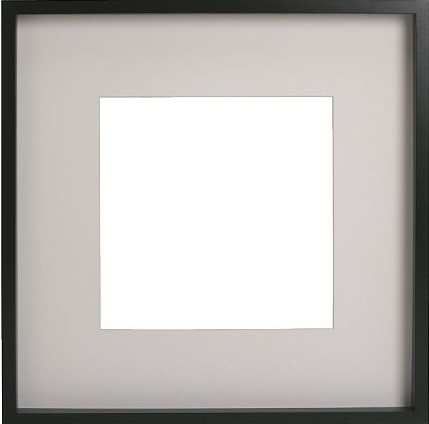
\includegraphics[scale=0.5]{bilder/ribba-rahmen-schwarz.jpg}
	\end{center}
	\caption{RIBBA Rahmen, schwarz}
	\vspace{-10pt}
\end{wrapfigure}
Bei der Auswahl des Spiegelrahmens haben wir uns lange Gedanken gemacht. Wir mussten nämlich die Entscheidung treffen ob wir den Rahmen von einem Schreiner anfertigen lassen, einen Rahmen selbst produzieren oder ein ähnliches Produkt unseren Bedürfnissen anpassen und somit umfunktionieren möchten. Die Auswahl des Rahmens ist eng mit der Auswahl des Spiegels verflochten. Das eine entscheidet das andere. Hat man bereits einen Spiegel erworben, bestimmt dieser die Größe des Rahmens. Natürlich hat man dadurch nicht mehr die Möglichkeit auf Fremdprodukte zurück zu greifen. Daher empfehlen wir zuerst die Anschaffung des Rahmens, um anschließend anhand der Rahmengröße den passenden Spiegel zu besorgen. \\
Die Herstellung durch ein Subunternehmen fiel ziemlich schnell aus der Wertung heraus, da es viel Geld kosten würde und wir unser Budget auf Grund der anderen Komponenten nicht überstrapazieren wollten. \\
Da uns nur eine begrenzte Zeit zur Verfügung stand und wir uns von Beginn an nicht sicher waren ob uns eine Eigenproduktion ästhetisch gefällt, haben wir uns für die dritte Option entschieden. \\
Nach einer kurzen Recherche haben wir den Tipp bekommen, dass der Bilderrahmen in Abbildung 2.1 der Firma IKEA genau unseren Bedürfnissen entspricht und sich somit ohne großen Aufwand umbauen ließe. \\
Die Größe des Rahmens ist 50 x 50 x 4,5 cm. Bedauerlicherweise stehen nicht genau 4,5 cm Höhe zur Verfügung, sondern nur ca 4 cm. Die Rückwand ist in den Rahmen integriert und hat uns somit kostbaren Platz geraubt. Nach dem ersten Abschätzen reichte uns die Größe jedoch aus und so haben wir uns gegen einen weiteren Umbau entschieden. \\ 
Die einzige Herausforderung bestand nun die restlichen Komponenten in der begrenzten Höhe unter zubringen. \\
Der Preis für den Rahmen lag lediglich bei 12,99 € und war somit einer der günstigsten Komponenten.

\subsection{Fazit}
Wenn man das Projekt schnell realisieren möchte, empfehlen wir definitiv die Verwendung des IKEA Rahmens. Zu beachten ist jedoch, dass die Wahl der Größe eingeschränkt ist. Hat man hingegen den Wunsch einen größeren Spiegel oder z.B. einen Spiegel für das Badezimmer mit Ablageflächen zu konstruieren, bleiben nur die beiden ersten Optionen übrig. Ist man Handwerklich begabt und hat man genügend Zeit, sowie Budget, kann man sicherlich den Bau des Rahmens selbstständig durchführen. Oder man lässt sich einen Rahmen nach seinen Bedürfnissen anfertigen. \\
Im nächsten Unterkapitel gehen wir näher auf die Eigenschaften des Spiegels ein und werden zum Ende von Kapitel 2 die Fertigung unseres \textit{SmartMirrors} erklären. 


\section{Der Spiegel}
Die Wahl des richtigen Spiegels ist entscheidend für die Funktion des \textit{SmartMirrors}. Ein weiterer Vorteil des IKEA Rahmens ist die Glasscheibe, die bereits beim Bilderrahmen mitgeliefert wird. \\
Ebenso wie bei dem Rahmen standen uns wieder zwei Optionen zur Verfügung. Entweder wir lassen uns den Spiegel professionell Beschichten oder wir kaufen eine sogenannte Spionfolie und bringen diese auf eine Glasscheibe auf. \\
Daher nutzten wir den bereits erwähnten Vorteil aus und entschieden uns für die eigene Folierung der vorhandenen Scheibe. Das ersparte uns Zeit und Geld, da die Folie nur \EUR{13,89} inkl. Versand kostete und die Glasscheibe innerhalb von 15 min foliert war.

\subsection{Das Folierwerkzeug}
Für die Folierung benötigt man zusätzlich noch 
\begin{center}
	\begin{singlespace}
		\begin{itemize}
			\item ein Folienrakel
			\item eine Sprühflasche mit einer Wasser-Spülmittellösung
			\item ein Cuttermesser
			\item ein Scheibentuch bzw. Microfasertuch, was am besten keine Fuseln hinterlässt.
		\end{itemize}
	\end{singlespace}
\end{center}
Hat man kein Folienrakel zur Verfügung, kann man sich einen unter folgendem \href{https://www.amazon.de/Folienrakel-Filzkante-Filzrakel-Kunststoffrakel-Verkleberakel/dp/B073S7KT25/ref=sr_1_2?ie=UTF8&qid=1503417838&sr=8-2&keywords=werkzeug+folierung}{Link} bei Amazon bestellen oder greift alternativ zu einer Kreditkarte. Diese wickelt man in ein Brillentuch ein und benutzt diese als Ersatz für den Folienrakel. Ersatzweise kann man statt dem Spülwasser auch Scheibenreiniger verwenden.

\newpage
\subsection{Die Folierung der Folie}
\begin{wrapfigure}{r}{0.5\textwidth}
	\vspace{-20pt}
	\begin{center}
		\includegraphics[scale=0.07]{bilder/spionspiegel.jpg}
	\end{center}
	\caption{Arbeitsbild der Folierung während des Proseminars}
	\vspace{-10pt}
\end{wrapfigure}
Um die Folie auf die Scheibe aufzutragen, sollte man diese zunächst gründlich reinigen und anschließend am besten mit einem Fensterwischer abziehen, um soviel Staub und Schmutz wie möglich abzutragen. Das beste Ergebnis lässt sich erzielen, wenn man den Vorgang im Badezimmer durchführt und kurz vorher heißes Wasser aus der Dusche laufen lässt. Das heiße Wasser erhöht die Luftfeuchtigkeit im Raum und senkt somit den Staubgehalt in der Luft, was optimal für unser Vorhaben ist. \\
Anschließend befeuchtet man leicht die Scheibe mit dem Spülwasser, um eine Art Gleitschicht zu erzeugen. Diese Gleitschicht erleichtert uns später das positionieren der Folie und minimiert die Bläschenbildung. Die Folie wird ,,schwimmend`` aufgetragen. \\
Meist ist die Folien mit einer Schutzschicht versehen. Um die Schutzschicht leichter von der Spionfolie zu lösen, nimmt man zwei Streifen Tesafilm und klebt diese auf eine Ecke von beiden Seiten auf. Beim auseinanderziehen lösen sich die beiden Folien von einander. Dabei ist zu beachten, dass man anschließend die richtige Seite zur weiteren Bearbeitung verwendet und diese nicht beim abziehen beschädigt. \\
Wir empfehlen definitiv etwas mehr Folie zur bestellen. Sollte beim Folieren etwas schief gehen, kann man diese einfach wieder abziehen und einen zweiten Versuch starten. Die Folie sollte idealerweise einige Zentimeter breiter und länger sein, als die Glasscheibe selbst. Da man die Folie zunächst positionieren muss, ist nicht zu vermeiden das Fingerabdrücke auf der Folie zusehen sind. Um diese zu entfernen, lässt man die Folie etwas überstehen und schneidet im Anschluss die Seiten mit einem Cuttermesser ab. \\
Für den nächsten Schritt sollte man sich am besten eine zweite Person als Unterstützung holen. Das erleichtert den Vorgang enorm. Nachdem die Folie von der Schutzschicht getrennt wurde, legt man diese auf einer Seite der Glasscheibe auf und rakelt die Luftbläschen mit Hilfe des Folienrakels von einer Seite zur anderen und von Innen nach außen heraus. Siehe Abbildung 2.3. Die Hilfsperson hält dabei die andere Seite der Folie etwas höher und straft diese nach Bedarf. Anschließend schneidet man die überstehenden Seiten vorsichtig und gleichmäßig ab und rakelt anschließend nochmal die Luftbläschen heraus. Ist man mit dem Ergebnis zufrieden, sollte man die Scheibe einen Tag liegen lassen, bevor man die Glasscheibe reinigt. Erfahrungsgemäß verflüchtigt sich das Wasser unter der Folie nach einigen Tagen. Die restlichen Luftbläschen sollten dann verschwunden sein.
\begin{figure}[H]
	\begin{center}
		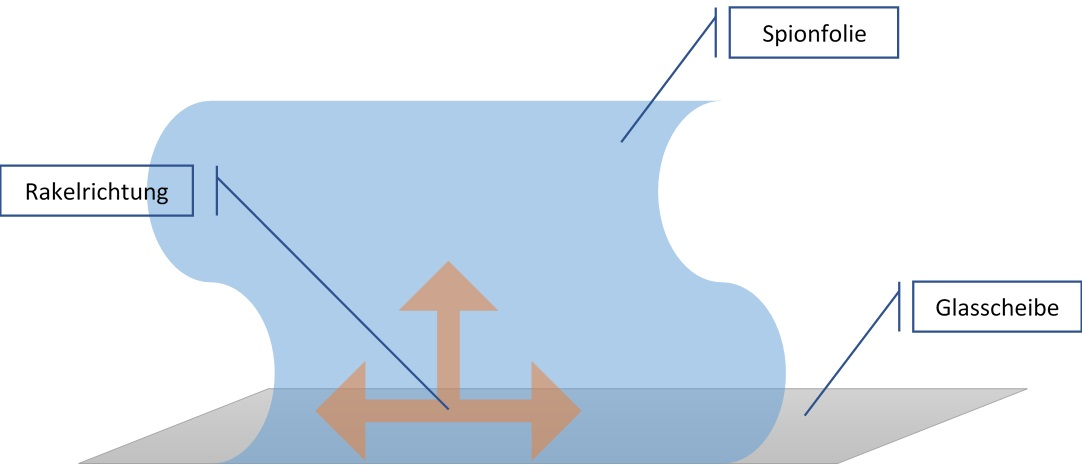
\includegraphics[scale=0.5]{bilder/Rakelanleitung.jpg}
	\end{center}
	\caption{Rakelrichtung}
\end{figure} 

\subsection{Der Spionspiegel}
Kurzer Hand möchten wir noch kurz auf die Eigenschaft des Spionspiegels, auch bekannt unter dem Namen Einwegspiegel, eingehen. Das Besondere daran ist, das der Spiegel von einer Seite bis zu einem bestimmten Prozentsatz reflektierend ist und von der anderen Seite Lichtdurchlässig, auch unter dem Begriff Transmission bekannt. Siehe Abbildung 2.2. Diese Eigenschaften ermöglichen es uns auf der Rückseite des Spiegels, also im Inneren, einen Monitor anzubringen dessen Licht auf der reflektierenden Seite angezeigt wird. Dabei entscheidet das Verhältnis zwischen dem Reflexionsgrad und der Transmission über die Qualität der Anzeige. Daher empfiehlt es sich einen Spiegel mit dem Reflexionsgrad von ca. 70-80\% und einem Transmissionswert von etwa 8\% zu verwenden. 
\begin{figure}[H]
	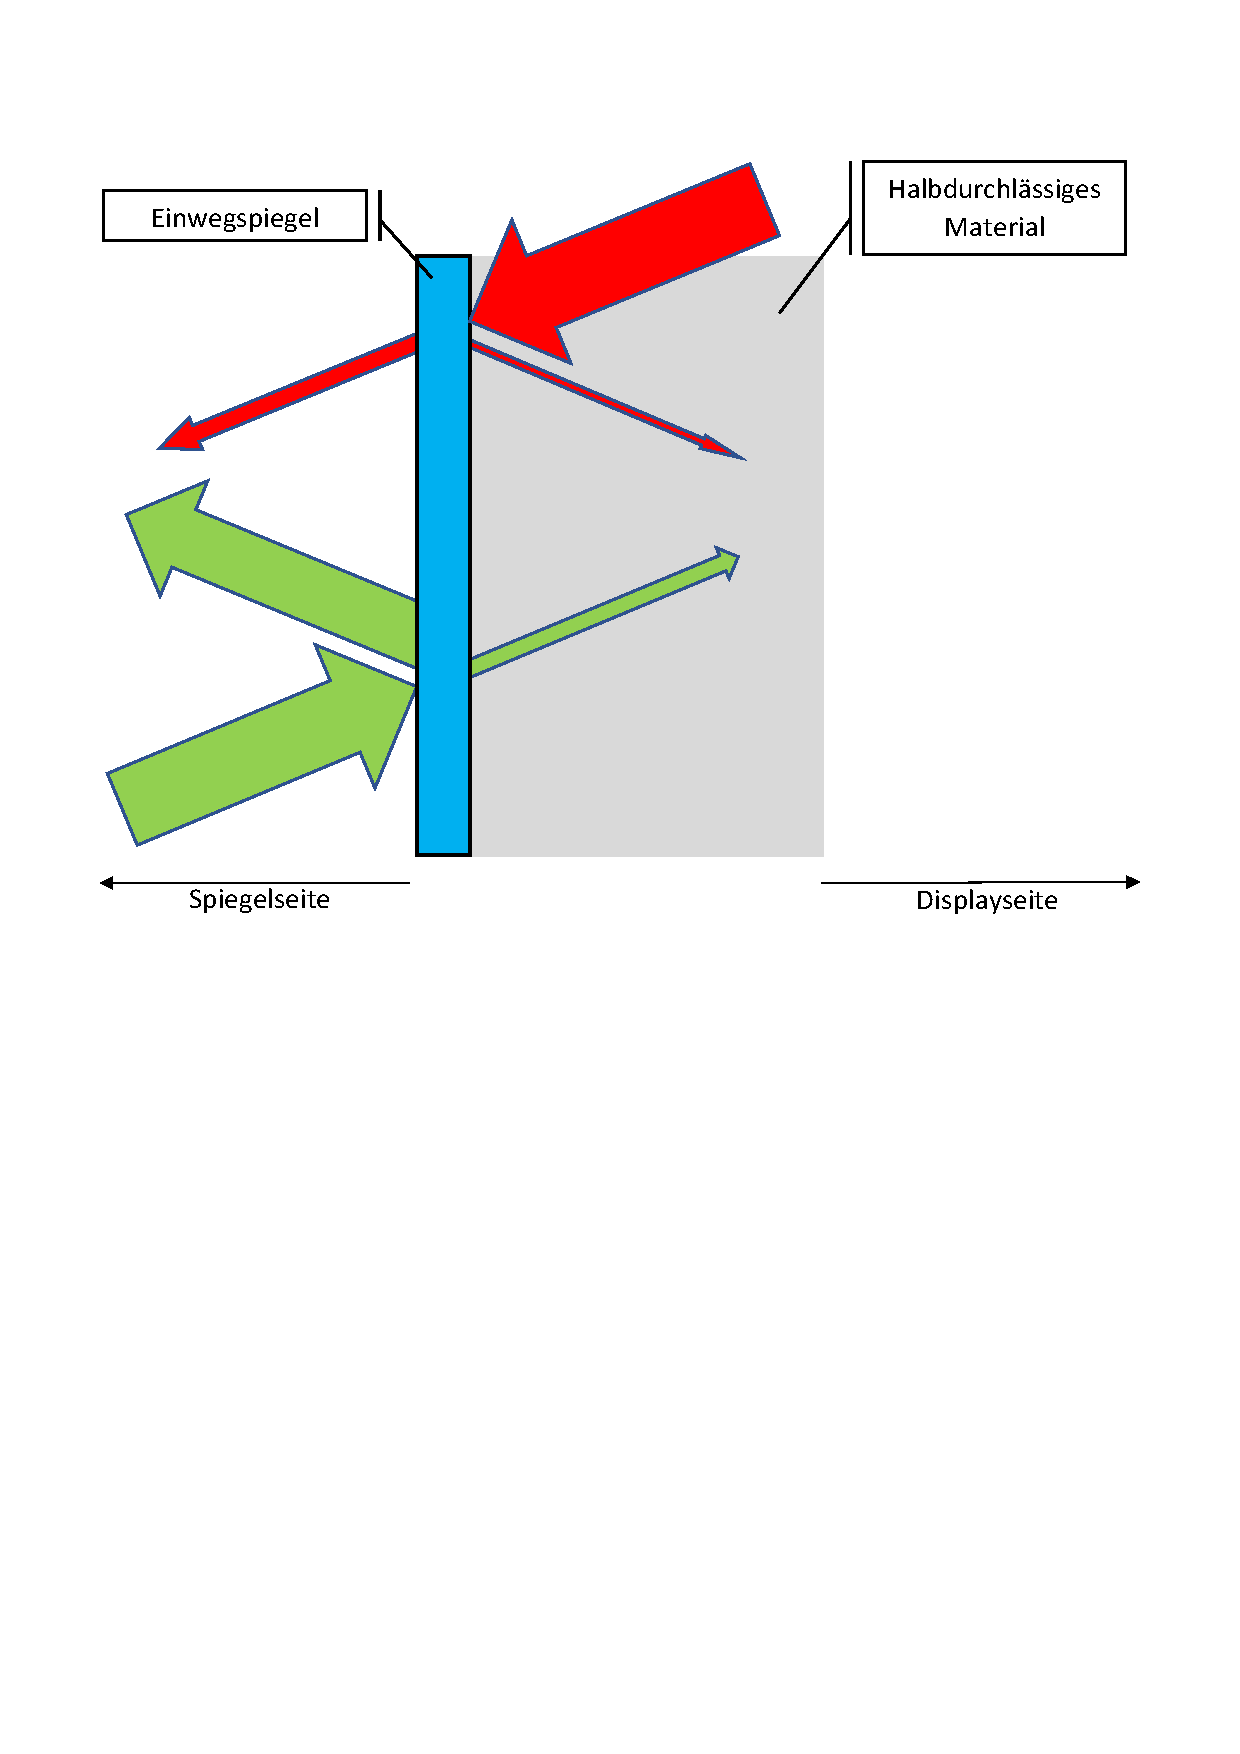
\includegraphics[trim=30mm 140mm 30mm 30mm, scale=0.5]{bilder/Einwegspiegel.pdf}\\
	\caption{Reflexions- und Transmissionswirkung}
	{\scriptsize Der rote Pfeil symbolisiert das Displaylicht und der grüne Pfeil das Umgebungslicht des Spiegels. Das Umgebungslicht wird zum größten Teil wieder reflektiert und das Displaylicht wird nahezu nach außen geleitet. }
\end{figure}

\subsection{Fazit}
Unser Fazit ist, dass sich die Verwendung einer Spionspiegelfolie eher mäßige bis geradeso akzeptable Qualität bietet. Um bessere Ergebnisse zu erzielen, sollte man am besten auf eine professionell beschichtete Glasscheibe zurückgreifen. Die Firma Glas Star aus Bochum hat sich auf die Herstellung der Glasscheiben für Smart Mirrors spezialisiert und bietet zahlreiche Auswahlmöglichkeiten. Die Webseite erreicht man unter dem folgenden \href{https://www.glas-star.de/spionspiegelnachmass/chrome-spy-spiegel/}{Link}. Der einzige Vorteil der Spionspiegelfolie war der zeitliche Aspekt und die vergleichsweise niedrigen Kosten.

\section{Das Innenleben}
\subsection{Raspberry Pi 3}
Als Steuereinheit haben wir uns für den Raspberry Pi 3 Model B entschieden. Aufgrund des integrierten WLAN-Moduls eignet sich der Raspberry Pi 3 ideal für unser Vorhaben. Der 
\textit{SmartMirror} kann somit mobil eingesetzt werden und ist nicht fest an einen Ort gebunden. \\
Für unser Projekt haben wir lediglich einige GPIO-Anschlüsse des Boards benötigt, um den Temperatur- und Bewegungsmeldersensor anzuschließen und zu verwenden. Die genau Belegung der GPIO-Anschlüsse findet man in Abbildung 2.5.
\begin{figure}[H]
	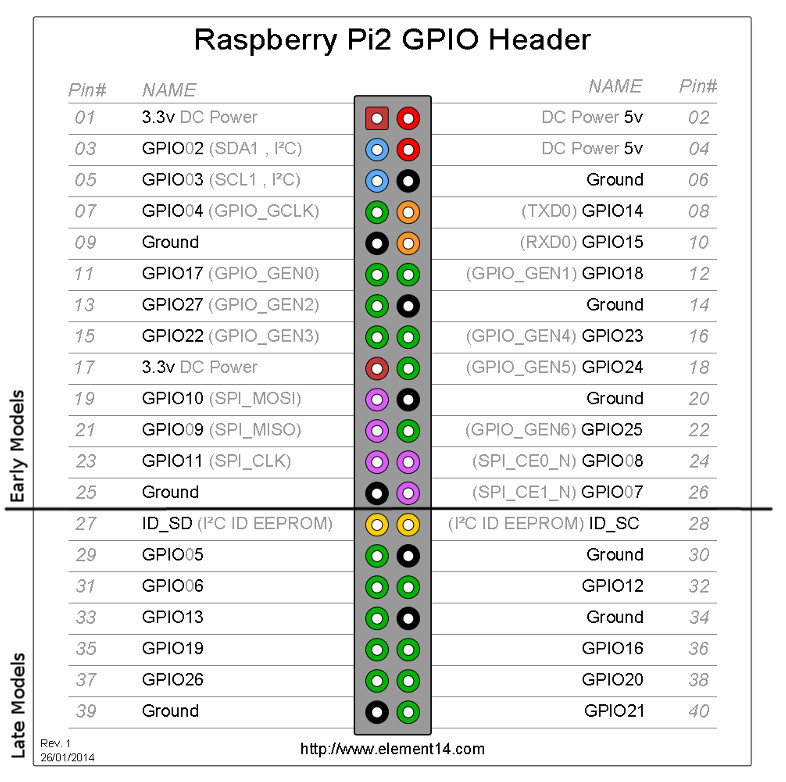
\includegraphics[scale=0.4]{bilder/gpio_pinout.jpg}
	\caption{GPIO-Belegung}
\end{figure}
Möchte man sich näher mit den Eigenschaften des Raspberry Pi beschäftigen, findet man unter \url{https://www.raspberrypi.org/documentation/} eine ausführliche Dokumentation. Da der Raspberry Pi üblicherweise ohne ein Betriebssystem geliefert wird, ist unter der genannten Adresse ebenfalls eine detaillierte Installationsanleitung zu finden.\\
Als Operating System haben wir die ,,RASPBIAN JESSIE WITH DESKTOP`` Distribution verwendet. Alternativ zur Desktop Version gibt es eine Light Version. Diese war für uns leider ungeeignet, da wir für unser Projekt eine grafische Oberfläche benötigen. Nähere Einzelheiten zu weiterer Software gibt es im Kapitel 3. \\


\subsection{Bewegungsmelder}
Als Bewegungssensor haben wir uns für den HC-SR501 entschieden. Der PIR-Sensor, oder auch ,,IR-Bewegungssensor`` genannt, arbeitet passiv auf Basis der Infrarotstrahlung der Umgebung.  Jeder Körper sendet eine kleine Menge an Infrarotstrahlung aus. Der PIR-Sensor stellt die Temperaturänderung im Raum fest und kann somit als Schalter verwendet werden. \\
Der Sensor befindet sich auf einer kleinen Platine und besitzt eine einstellbare Empfindlichkeit und zwei M2 Befestigungsbohrungen für die Montage. Die Reichweite der Erfassung beträgt bis zu 7 Meter. Der Erfassungswinkel des Objektives beträgt etwa 100 Grad. \\
Der Sensor ermöglicht es uns je nach Bedarf das Display an zusteuern und somit Energie zu sparen. Betritt eine Person den Raum, indem der Spiegel hängt, gibt der Sensor ein Signal und wir können das Display einschalten. Dazu verbindet wir den PIR-Sensor mit dem Ein-/Ausschalter des Monitors. Andernfalls bleibt das Display ausgeschaltet. \\

Zum anschließen des Sensors an den Raspberry Pi 3 benötigt man zusätzlich drei Jumperkabel. Alternativ dazu verwendet man ein dreiadriges Kabel und verbindet die Anschlüsse wie folgt. Diese sind auf dem Sensor beschriftet. 
\begin{center}
	\begin{singlespace}
		\begin{itemize}
			\item VCC an Pin 2 (5V)
			\item OUT an Pin 16 (GPIO 23)
			\item GND an Pin 6 (Ground)
		\end{itemize}
	\end{singlespace}
\end{center} 
\begin{figure}[H]
	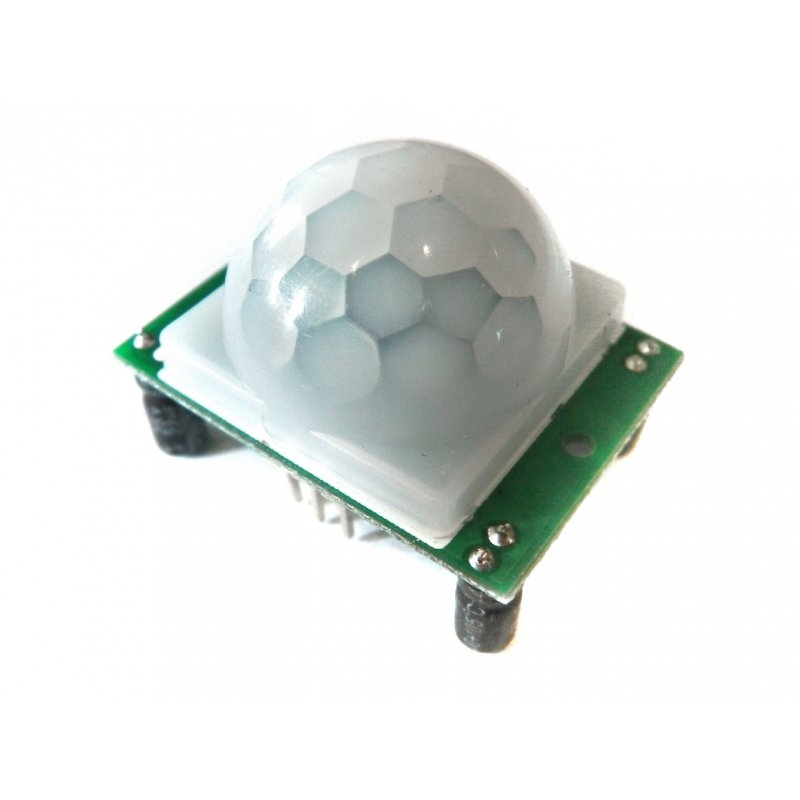
\includegraphics[trim=20mm 20mm 20mm 20mm, scale=0.2]{bilder/PIR-Sensor.jpg}
	\caption{PIR-Sensor HC-SR501}
\end{figure}

\subsection{Temperatur- und Luftfeuchtigkeitssensor}


\newpage
\section{Konstruktions-Skizze}
\begin{figure}[H]
		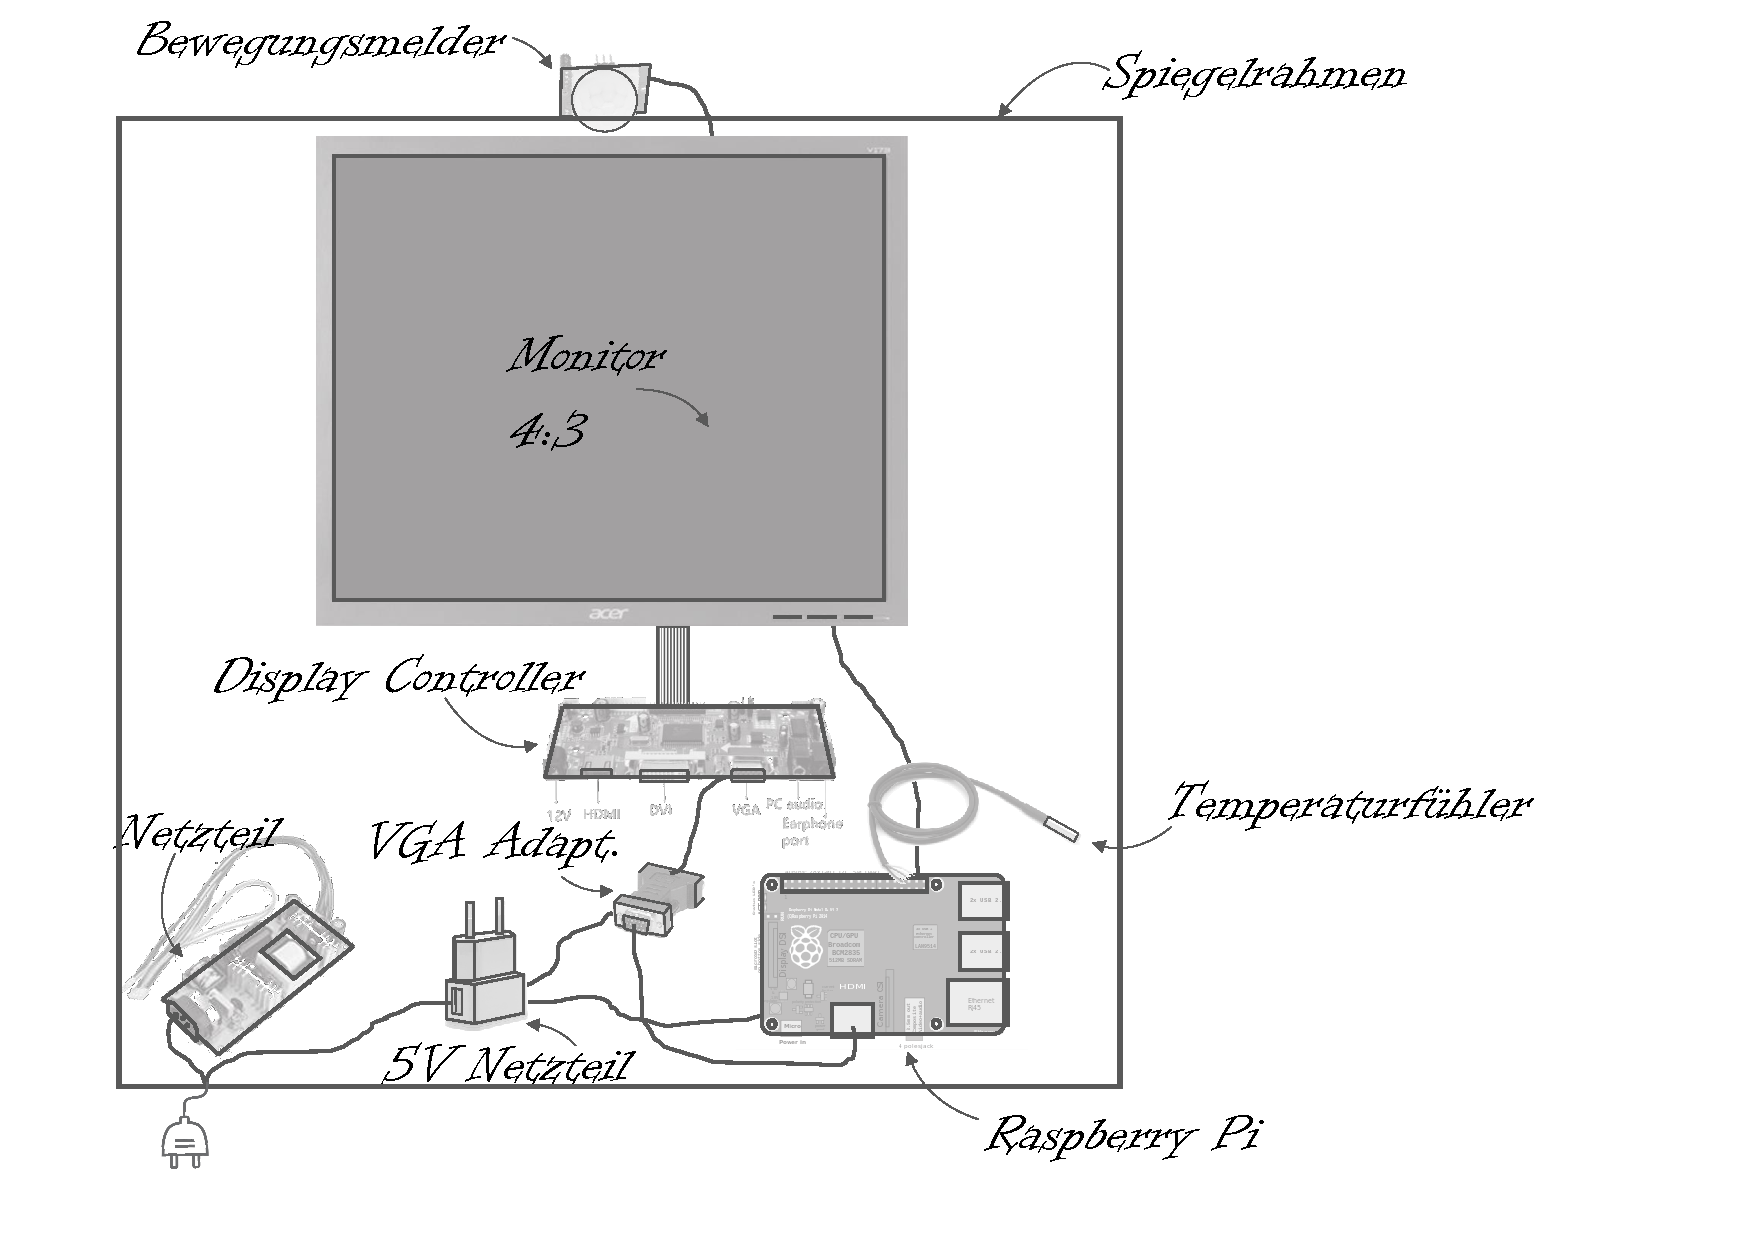
\includegraphics[scale=0.5, trim=0mm 10mm 85mm 10mm]{bilder/smartMirrorExplosionsskizze.pdf}
	\caption{Anordnung und Verkabelung der Komponenten}
\end{figure}

\section{Die Fertigung}
\section{Ein weiteres Unterkapitel}